\scanpage{18}
Donc le choix \inserted{\text{supplémentaire}} de $s_0$ est le choix d'un pt sur une droite \inserted{\text{$D_\sigma$}}. Il faudra de plus, tout d'abord $s_0\ne us_0$, \deleted{\unsure{don|dire} $s_0\notin D_{\sigma'}$} ou ce qui revient au $=$ (\unsure{introduisant|introduisons} \unsure{l'élém|l'élémt} $\sigma'=\deleted{\unsure{\sigma}}u\sigma$ tel que $u=\sigma'\sigma$ -- la symétr. \unsure{bissec.} fixant $(s_0,s_1)$) que $s_0\ne\sigma's_0$ i.e.
\[
s_0\notin D_\sigma\cap D_{\sigma'}
\]

\figure{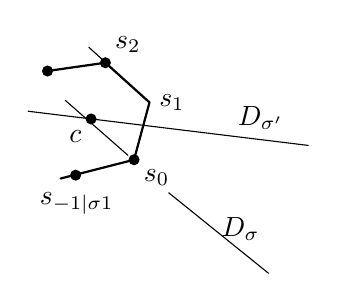
\begin{tikzpicture}[x=.7cm,y=.7cm,line cap=round,line join=round]
\draw[thick] (.35,3.55)--(1.40,3.7)--(2.2,2.98)--(1.92,1.94)--(.59,1.60);
\draw (.0,2.82)--(5.08,2.20) node[pos=.83,above] {$D_{\sigma'}$};
\draw (.67,3.02)--(1.81,2.02);
\draw (2.55,1.34)--(4.36,-.12) node[pos=.72,above] {$D_\sigma$};
\draw (1.10,3.98)--(1.52,3.60);
\foreach \x/\y in {.35/3.55,1.40/3.7,1.92/1.94,.86/1.66,1.14/2.68}{\fill (\x,\y) circle (2pt);}
\node[above right] at (1.40,3.7) {$s_2$};
\node[right] at (2.2,2.98) {$s_1$};
\node[below right] at (1.92,1.94) {$s_0$};
\node[below] at (.88,1.52) {$s_{\unsure{-1|\sigma1}}$};
\node[below left] at (1.14,2.65) {$c$};
\end{tikzpicture}}

[Nb \deleted{\unsure{à trouver}} $D_{\sigma'}$ est l'ens des pts fixes de $\sigma'$] -- On trouvera que les conditions à imposer à $\varphi$ pour qu'il y ait $s_0$ satisfaisant ttes les conditions impliquent que \deleted{\unsure{$D_{\sigma'}$}} $\sigma'$ est également une réflexion et $D_\sigma\ne D_{\sigma'}$ -- donc \deleted{\unsure{pour}} celà exclut \inserted{\text{a priori}} en plus un pt $c$ (le \uline{centre} du polygône \inserted{\text{qui est un pt fixe \unsure{sous|pour} $\varphi(D_n)$}}) parmi les pts éligibles pour $s_0$. On trouvera de plus que (pour $\varphi$ fixé, \deleted{les ens des pts $s$} \inserted{\text{\uline{admissible}}}) l'ens des $s_0\in\deleted{\unsure{tels}}D^{\sigma *}$ $=$ \deleted{distincts de} $D^\sigma-\{D\cap D^\sigma\}$ \deleted{\unsure{est un}} -- sur le quel le commutant \inserted{\text{$G$}} de $\varphi(\Gamma)$ dans $\mathrm{Aff}(E)$ opère de façon évidente) est un \uline{torseur} sous $G$.
% archive sheet number: 17
